\documentclass{standalone}
\usepackage{tikz}
\usetikzlibrary{patterns, positioning}


\begin{document}
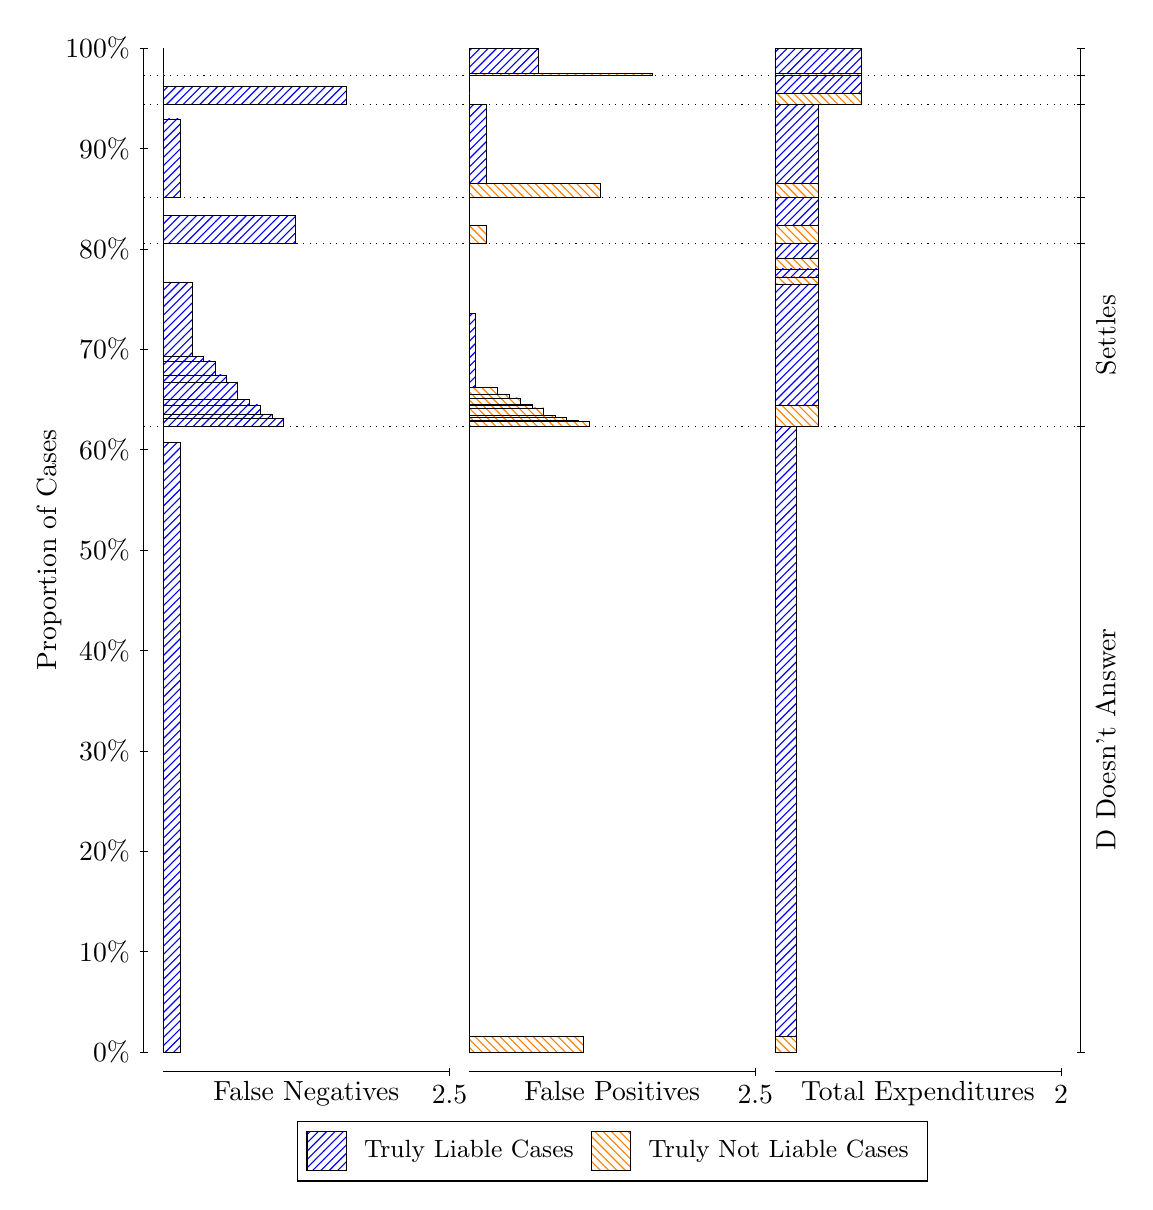
\begin{tikzpicture}
\draw[black, very thin] (1.5,1.75) -- (1.5,14.5);
\node[rotate=90, text=black, anchor=center] at (0.3, 8.125) {Proportion of Cases};
\draw[black, very thin] (1.45,1.75) -- (1.55,1.75);
\node[text=black, anchor=east] at (1.45, 1.75) {0\%};
\draw[black, very thin] (1.45,3.025) -- (1.55,3.025);
\node[text=black, anchor=east] at (1.45, 3.025) {10\%};
\draw[black, very thin] (1.45,4.3) -- (1.55,4.3);
\node[text=black, anchor=east] at (1.45, 4.3) {20\%};
\draw[black, very thin] (1.45,5.575) -- (1.55,5.575);
\node[text=black, anchor=east] at (1.45, 5.575) {30\%};
\draw[black, very thin] (1.45,6.85) -- (1.55,6.85);
\node[text=black, anchor=east] at (1.45, 6.85) {40\%};
\draw[black, very thin] (1.45,8.125) -- (1.55,8.125);
\node[text=black, anchor=east] at (1.45, 8.125) {50\%};
\draw[black, very thin] (1.45,9.4) -- (1.55,9.4);
\node[text=black, anchor=east] at (1.45, 9.4) {60\%};
\draw[black, very thin] (1.45,10.675) -- (1.55,10.675);
\node[text=black, anchor=east] at (1.45, 10.675) {70\%};
\draw[black, very thin] (1.45,11.95) -- (1.55,11.95);
\node[text=black, anchor=east] at (1.45, 11.95) {80\%};
\draw[black, very thin] (1.45,13.225) -- (1.55,13.225);
\node[text=black, anchor=east] at (1.45, 13.225) {90\%};
\draw[black, very thin] (1.45,14.5) -- (1.55,14.5);
\node[text=black, anchor=east] at (1.45, 14.5) {100\%};

\draw[black, very thin] (13.4,1.75) -- (13.4,14.5);
\draw[black, very thin] (13.35,1.75) -- (13.45,1.75);
\node[anchor=west] at (13.35, 1.75) {};
\draw[black, very thin] (13.35,9.6931) -- (13.45,9.6931);
\node[anchor=west] at (13.35, 9.6931) {};
\draw[black, very thin] (13.35,12.019) -- (13.45,12.019);
\node[anchor=west] at (13.35, 12.019) {};
\draw[black, very thin] (13.35,12.599) -- (13.45,12.599);
\node[anchor=west] at (13.35, 12.599) {};
\draw[black, very thin] (13.35,13.782) -- (13.45,13.782);
\node[anchor=west] at (13.35, 13.782) {};
\draw[black, very thin] (13.35,14.152) -- (13.45,14.152);
\node[anchor=west] at (13.35, 14.152) {};
\draw[black, very thin] (13.35,14.5) -- (13.45,14.5);
\node[anchor=west] at (13.35, 14.5) {};

\draw[black, very thin, pattern color=blue, pattern=north east lines] (1.75,1.75) rectangle (1.968,9.4921);
\draw[black, very thin, pattern color=orange, pattern=north west lines] (1.75,9.4921) rectangle (1.75,9.6931);
\draw[black, very thin, pattern color=blue, pattern=north east lines] (1.75,9.6931) rectangle (3.276,9.7941);
\draw[black, very thin, pattern color=blue, pattern=north east lines] (1.75,9.7941) rectangle (3.1307,9.8508);
\draw[black, very thin, pattern color=blue, pattern=north east lines] (1.75,9.8508) rectangle (2.9853,9.9675);
\draw[black, very thin, pattern color=blue, pattern=north east lines] (1.75,9.9675) rectangle (2.84,10.039);
\draw[black, very thin, pattern color=blue, pattern=north east lines] (1.75,10.039) rectangle (2.6947,10.254);
\draw[black, very thin, pattern color=blue, pattern=north east lines] (1.75,10.254) rectangle (2.5493,10.35);
\draw[black, very thin, pattern color=blue, pattern=north east lines] (1.75,10.35) rectangle (2.404,10.527);
\draw[black, very thin, pattern color=blue, pattern=north east lines] (1.75,10.527) rectangle (2.2587,10.584);
\draw[black, very thin, pattern color=blue, pattern=north east lines] (1.75,10.584) rectangle (2.1133,11.519);
\draw[black, very thin, pattern color=orange, pattern=north west lines] (1.75,11.519) rectangle (1.75,12.019);
\draw[black, very thin, pattern color=blue, pattern=north east lines] (1.75,12.019) rectangle (3.4213,12.371);
\draw[black, very thin, pattern color=orange, pattern=north west lines] (1.75,12.371) rectangle (1.75,12.599);
\draw[black, very thin, pattern color=blue, pattern=north east lines] (1.75,12.599) rectangle (1.968,13.601);
\draw[black, very thin, pattern color=orange, pattern=north west lines] (1.75,13.601) rectangle (1.75,13.782);
\draw[black, very thin, pattern color=blue, pattern=north east lines] (1.75,13.782) rectangle (4.0753,14.011);
\draw[black, very thin, pattern color=orange, pattern=north west lines] (1.75,14.011) rectangle (1.75,14.152);
\draw[black, very thin, pattern color=orange, pattern=north west lines] (1.75,14.152) rectangle (1.75,14.177);
\draw[black, very thin, pattern color=blue, pattern=north east lines] (1.75,14.177) rectangle (1.75,14.5);
\draw[black, very thin, pattern color=orange, pattern=north west lines] (5.6333,1.75) rectangle (7.0867,1.951);
\draw[black, very thin, pattern color=blue, pattern=north east lines] (5.6333,1.951) rectangle (5.6333,9.6931);
\draw[black, very thin, pattern color=orange, pattern=north west lines] (5.6333,9.6931) rectangle (7.1593,9.7535);
\draw[black, very thin, pattern color=orange, pattern=north west lines] (5.6333,9.7535) rectangle (7.014,9.7664);
\draw[black, very thin, pattern color=orange, pattern=north west lines] (5.6333,9.7664) rectangle (6.8687,9.8062);
\draw[black, very thin, pattern color=orange, pattern=north west lines] (5.6333,9.8062) rectangle (6.7233,9.8333);
\draw[black, very thin, pattern color=orange, pattern=north west lines] (5.6333,9.8333) rectangle (6.578,9.9292);
\draw[black, very thin, pattern color=orange, pattern=north west lines] (5.6333,9.9292) rectangle (6.4327,9.9676);
\draw[black, very thin, pattern color=orange, pattern=north west lines] (5.6333,9.9676) rectangle (6.4327,9.973);
\draw[black, very thin, pattern color=orange, pattern=north west lines] (5.6333,9.973) rectangle (6.2873,10.058);
\draw[black, very thin, pattern color=orange, pattern=north west lines] (5.6333,10.058) rectangle (6.142,10.104);
\draw[black, very thin, pattern color=orange, pattern=north west lines] (5.6333,10.104) rectangle (5.9967,10.193);
\draw[black, very thin, pattern color=blue, pattern=north east lines] (5.6333,10.193) rectangle (5.706,11.128);
\draw[black, very thin, pattern color=blue, pattern=north east lines] (5.6333,11.128) rectangle (5.6333,12.019);
\draw[black, very thin, pattern color=orange, pattern=north west lines] (5.6333,12.019) rectangle (5.8513,12.247);
\draw[black, very thin, pattern color=blue, pattern=north east lines] (5.6333,12.247) rectangle (5.6333,12.599);
\draw[black, very thin, pattern color=orange, pattern=north west lines] (5.6333,12.599) rectangle (7.3047,12.78);
\draw[black, very thin, pattern color=blue, pattern=north east lines] (5.6333,12.78) rectangle (5.8513,13.782);
\draw[black, very thin, pattern color=orange, pattern=north west lines] (5.6333,13.782) rectangle (5.6333,13.923);
\draw[black, very thin, pattern color=blue, pattern=north east lines] (5.6333,13.923) rectangle (5.6333,14.152);
\draw[black, very thin, pattern color=orange, pattern=north west lines] (5.6333,14.152) rectangle (7.9587,14.177);
\draw[black, very thin, pattern color=blue, pattern=north east lines] (5.6333,14.177) rectangle (6.5053,14.5);
\draw[black, very thin, pattern color=orange, pattern=north west lines] (9.5167,1.75) rectangle (9.7892,1.951);
\draw[black, very thin, pattern color=blue, pattern=north east lines] (9.5167,1.951) rectangle (9.7892,9.6931);
\draw[black, very thin, pattern color=orange, pattern=north west lines] (9.5167,9.6931) rectangle (10.062,9.9676);
\draw[black, very thin, pattern color=blue, pattern=north east lines] (9.5167,9.9676) rectangle (10.062,11.506);
\draw[black, very thin, pattern color=orange, pattern=north west lines] (9.5167,11.506) rectangle (10.062,11.594);
\draw[black, very thin, pattern color=blue, pattern=north east lines] (9.5167,11.594) rectangle (10.062,11.695);
\draw[black, very thin, pattern color=orange, pattern=north west lines] (9.5167,11.695) rectangle (10.062,11.832);
\draw[black, very thin, pattern color=blue, pattern=north east lines] (9.5167,11.832) rectangle (10.062,12.019);
\draw[black, very thin, pattern color=orange, pattern=north west lines] (9.5167,12.019) rectangle (10.062,12.247);
\draw[black, very thin, pattern color=blue, pattern=north east lines] (9.5167,12.247) rectangle (10.062,12.599);
\draw[black, very thin, pattern color=orange, pattern=north west lines] (9.5167,12.599) rectangle (10.062,12.78);
\draw[black, very thin, pattern color=blue, pattern=north east lines] (9.5167,12.78) rectangle (10.062,13.782);
\draw[black, very thin, pattern color=orange, pattern=north west lines] (9.5167,13.782) rectangle (10.607,13.923);
\draw[black, very thin, pattern color=blue, pattern=north east lines] (9.5167,13.923) rectangle (10.607,14.152);
\draw[black, very thin, pattern color=orange, pattern=north west lines] (9.5167,14.152) rectangle (10.607,14.177);
\draw[black, very thin, pattern color=blue, pattern=north east lines] (9.5167,14.177) rectangle (10.607,14.5);
\draw[black, dotted] (1.5,9.6931) -- (13.4,9.6931);
\draw[black, dotted] (1.5,12.019) -- (13.4,12.019);
\draw[black, dotted] (1.5,12.599) -- (13.4,12.599);
\draw[black, dotted] (1.5,13.782) -- (13.4,13.782);
\draw[black, dotted] (1.5,14.152) -- (13.4,14.152);
\draw[black, very thin] (1.75,1.5) -- (5.3833,1.5);
\node[text=black, anchor=north] at (3.5667, 1.5) {False Negatives};
\draw[black, very thin] (5.3833,1.45) -- (5.3833,1.55);
\node[text=black, anchor=north] at (5.3833, 1.45) {2.5};

\draw[black, very thin] (5.6333,1.5) -- (9.2667,1.5);
\node[text=black, anchor=north] at (7.45, 1.5) {False Positives};
\draw[black, very thin] (9.2667,1.45) -- (9.2667,1.55);
\node[text=black, anchor=north] at (9.2667, 1.45) {2.5};

\draw[black, very thin] (9.5167,1.5) -- (13.15,1.5);
\node[text=black, anchor=north] at (11.333, 1.5) {Total Expenditures};
\draw[black, very thin] (13.15,1.45) -- (13.15,1.55);
\node[text=black, anchor=north] at (13.15, 1.45) {2};

\node[text=black, centered, rotate=90] at (13.72, 5.7215) {D Doesn't Answer};
\node[text=black, centered, rotate=90] at (13.72, 10.856) {Settles};





\draw (7.449999999999999,1.5) node[draw=none] (baseCoordinate) {};
\begin{scope}[align=center]
        \matrix[scale=0.5, draw=black, below=0.5cm of baseCoordinate, nodes={draw}, column sep=0.1cm]{
            \node[rectangle, draw, minimum width=0.5cm, minimum height=0.5cm, pattern color=blue, pattern=north east lines] {}; &
            \node[draw=none, font=\small, text=black] (B) {Truly Liable Cases}; &
            \node[rectangle, draw, minimum width=0.5cm, minimum height=0.5cm, pattern color=orange, pattern=north west lines] {}; &
            \node[draw=none, font=\small, text=black] (B) {Truly Not Liable Cases}; \\
            };
\end{scope}

\end{tikzpicture}
\end{document}